\documentclass[11pt]{article}

    \usepackage[breakable]{tcolorbox}
    \usepackage{parskip} % Stop auto-indenting (to mimic markdown behaviour)
    \usepackage{caption}
    \DeclareCaptionFormat{nocaption}{}
    \captionsetup{format=nocaption,aboveskip=0pt,belowskip=0pt}
    \usepackage{float}
    \usepackage{xcolor}
    \usepackage{enumerate}
    \usepackage{geometry}
    \usepackage{amsmath}
    \usepackage{amssymb}

\begin{document}
    
\section{Tidal Evolution of the Earth Moon
System}\label{Introduction}

    For this project, python code was written to integrate the evolution of
the earth and moon from when they were formed to the present day. The
overall goal should show that about a billion years in the past, the two
bodies collided, ie the earth moon separation goes to zero.
\newpage
\section{Questions}
\subsection{Question 1}\label{question-1}

    For question one,the objective was to calculate The orbital angular
momentum of the earth($L_e$), The spin angular momentum of the earth($S_e$)
and the The orbital angular momentum of the moon($L_m$).

The orbital angular momentum of the earth is givens as:\\
$L_e=M_e\sqrt{(G(M_s+M_e)a_e)}\\
L_e=5.97*10^{27}\sqrt{(6.67×10^{-8}-1.9885×10^{33}+5.97×10^{27})*1.49×10^{11}}\\
L_e=2.653956693×10^{46}gcm^2s^{-1}$

This is the angular momentum of the earth due to its revolution. It is
calculated through L = mvr Where m = mass of the earth v = velocity of
the earth, r = the radius of the orbit The formula
considers the earth as a point of mass for circular orbit.

The spin angular momentum of the earth is given as:\\
$S_e=0.3299*M_eR_e^2\Omega_e\\
S_e=0.3299×5.97*10^{27}*6371000^2*7.29*10^{-5}\\
S_e=5.8294×10^{36}gcm^2s^{-1}$\\

This value is given by the
earth's moment of inertia mulitipied by the angular velocity of the
earth. It is as a result of the earth spinning around it's own axis
which generates momentum due to it's weight and velocity.

The orbital angular momentum of the moon is givens as:\\
$L_m=M_m\sqrt{(G(M_e+M_m)a_m)}\\
L_m=7.349×10^{25}\sqrt{(6.67*10^{-8}*(5.97*10^{27}+7.349×10^{25})*3.34*10^8)}\\
L_m=2.696548908*10^{40}gcm^2s^{-1}$

This momentum comes from the moons orbiting around the earth. The Moon
is a uniformly dense sphere (it isn't) of radius a $1.7375*10^3 km$, The
Moon's mass M is $7.3459*10^{22} kg$, The Moon's orbital period T is 27.322
days, or $2.3606*10^6 s$, The Moon's rotational period T is 27.322 days, or
$2.3606*10^6 s$, and The Moon's orbit is circular (it isn't), and is 385,000
km in radius r. The moon's angular velocity (both for its orbit and its
rotation, since its tidally locked in a 1:1 orbit)
\newpage
\subsection{Question 2}\label{question-2}

    Tidal torque of the earth is the result of adding tidal force on the
mass of the earth caused by tidal waves brought about by the earth-moon
relation. This is enough to significantly reduce the angualr velocity of
the earth. It is given by:\\
$T_e=\frac{3GM_e^{2}}{2a_e}(\frac{R_e}{a_e})^2\frac{K_2}{Q_e}
T_e =-4.94x10^{15}Nm$\\
\\
The tidal torque due to the moon is given by :\\
$T_m=\frac{3GM_m^{2}}{2a_m}(\frac{R_m}{a_m})^2\frac{K_2}{Q_m} 
T_m=2.5695×10^{31}gcm^2s^{-2}$

\newpage
\subsection{Question 3}\label{question-3}

From equation 1 time scale is $\frac{L_e}{T_s}=4.854×10^{15}s=153.919$million years 
From equation 2 time scale is $\frac{S_e}{T_s+T_m}=-187067.45s=-0.00593$ years 
From equation 3 time scale is $\frac{L_m}{T_m}=1.049×10^9s=33years$

\newpage
\subsection{Question 6}\label{question-6}
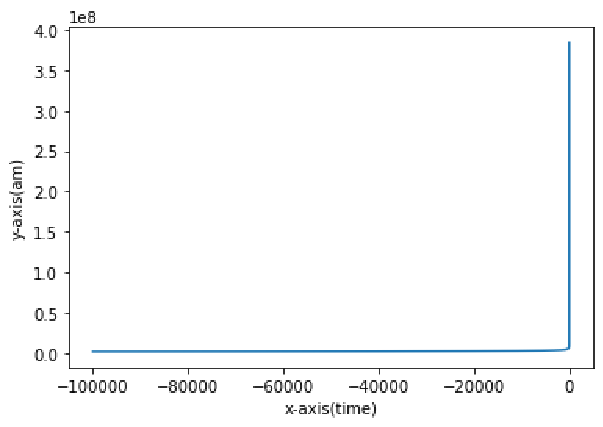
\includegraphics[]{output.png}

\newpage
\subsection{Question 8}\label{question-8}

    Roche Radius is the distance from a celestial body, within which a
secondary celestial body will begin to distintegrate as a result of the
former celestial body tidal forces being in excess of the secondary's
body gravitational attraction.\\
$A_c=2.44(\frac{M_e}{M_m})^{\frac{1}{3}}\frac{R_m^2}{R_e}\\
A_c=5000km$

The Roche radius is given by 9492 km / 5000 km = 1.8984 This means that
the length of the day was about 2 hours

\newpage
\subsection{Question 9}\label{question-9}

    The age of Earth is estimated to be 4.54 billion years with an accuracy
of + or - 50 million years. The Moon is speculated to be 4.53 billion
years old. The moon is considered to be a part of the earth that
detached itself post collision between the earth and another celestial
body. This only occured when the earth was 50 million years old which is
reflctive of the earth's age in relation to the moon. Here it is noted
that the two bodies are older than as expressed by the tidal wave
equations. The moons age can be used to tell how old the earth is.

    
\end{document}
